

\begin{figure}[t]
\centering
\begin{tabular} {
    c@{\hspace{1.0pt}} @{\hspace{1.0pt}}
    c@{\hspace{1.0pt}} @{\hspace{1.0pt}}
}
    
    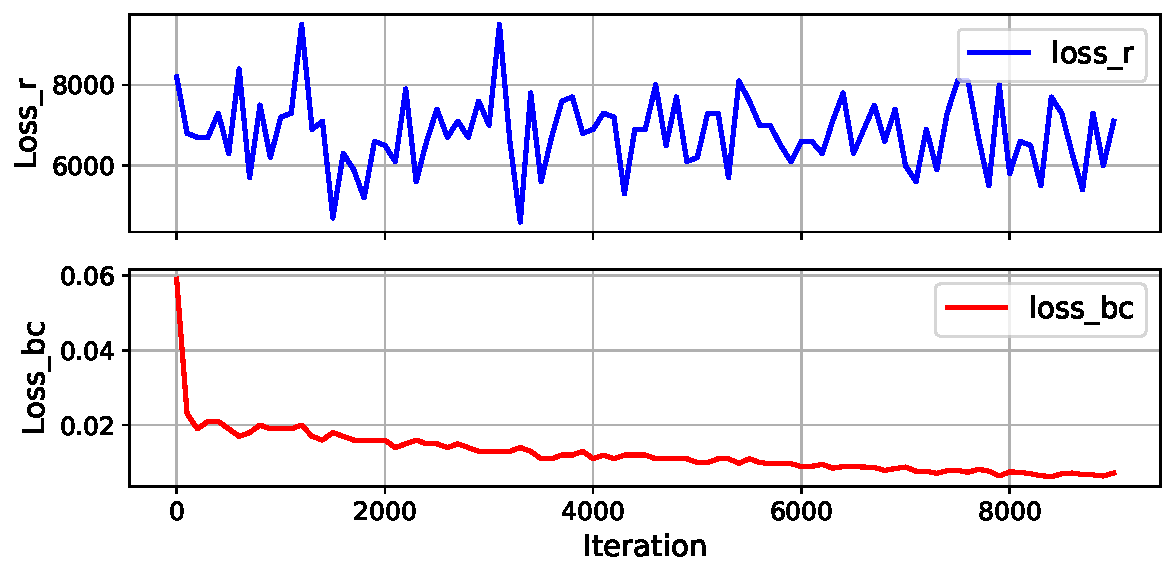
\includegraphics[width=0.45\columnwidth, trim={0.35cm 0.35cm 0.20cm 0.25cm}, clip]{figures/loss_plots_helmholtz.pdf} &
    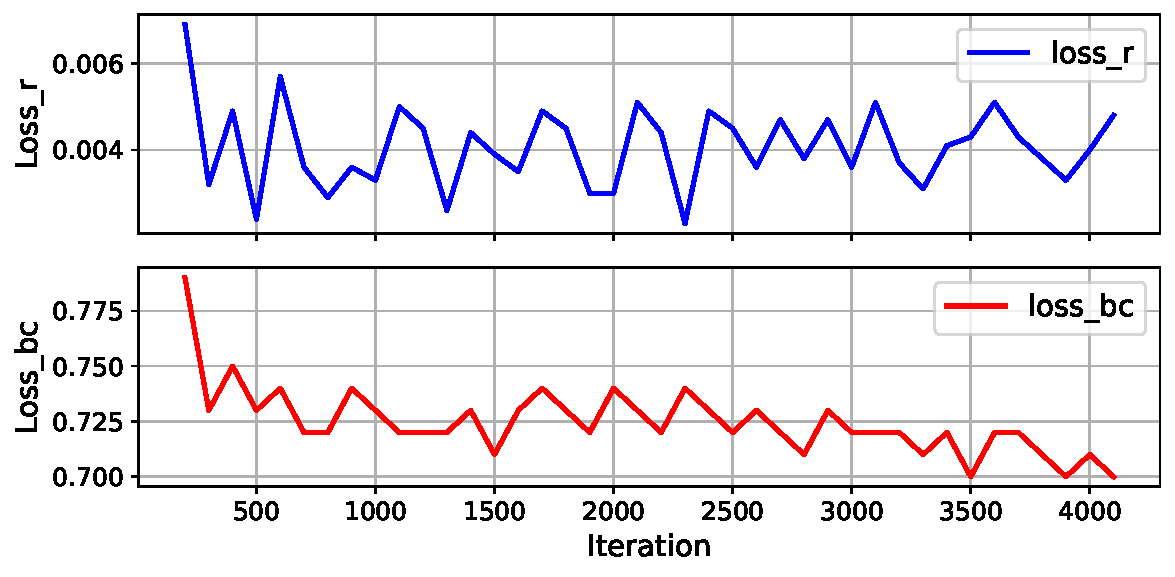
\includegraphics[width=0.45\columnwidth,trim={0.15cm 0.35cm 0.20cm 0.25cm}, clip]{figures/loss_plots_cavity.pdf} \\
    \footnotesize{(a) Helmholtz}  & \footnotesize{(b) Cavity} \\
    
\end{tabular}
\caption{Loss history behaviour of the CV-based QCPINN model when solving Helmholtz(a) and Cavity (b). ``loss\_r'' and ``loss\_bc'' refers to physical and boundary losses respectively.  While the ``loss\_bc'' demonstrates a clear decreasing trend, indicating improvements in satisfying the boundary conditions, the ``loss\_r'' exhibits significant fluctuations and does not show a noticeable reduction, suggesting challenges in minimizing the residual error of the governing equation.
}

\label{fig:cv_loss_plots}
\end{figure}


\begin{table}[t]
\centering
\caption{Performance comparison of different quantum and classical methods for the Helmholtz problem (\ref{eq:Helmholtz}). The table presents the number of trainable parameters, relative $L_2$ error (\%), final training loss, and the number of iterations required for convergence.}
\label{tab:results_helmholtz}
\scriptsize
\begin{tabular}{@{}l
        c@{\hspace{14.0pt}}
        c@{\hspace{4.0pt}}@{\hspace{4.0pt}} |
        c@{\hspace{14.0pt}}
        c@{\hspace{14.0pt}}
        c@{\hspace{14.0pt}}
        c@{\hspace{14.0pt}}
        @{}}
        \toprule
 \multicolumn{3}{c|}{\textbf{Method}} &\textbf{\makecell{\# Trainable \\Parameters}} & \multicolumn{2}{l}\textbf{\makecell{Relative $L_2$\\ Error(\%)}} & \textbf{\makecell{Final Training\\  Loss}}  \\
\midrule
  % \multirow{4}{*}{CV} & \multicolumn{2}{c|}{ \multirow{2}{*}{Algorithm(\ref{alg:algorithm1})}} & \multirow{2}{*}{469} & u & $1.00e+02 $  & \multirow{2}{*}{5077.79} & \multirow{2}{*}{20000}\\
  %                          &     &  & &   f &  $1.00e+02 $ & &  \\
  %       \cline{2- 7} \noalign{\vskip 1ex}
  %                          &      \multicolumn{2}{c|}{ \multirow{2}{*}{Algorithm(2)}} & 573 & u & $ 9.98e+01$&  \multirow{2}{*}{8068.73} &  \multirow{2}{*}{4200}\\
  %                          &     &  & &  f &  $9.95e+01$ & &  \\
  %      \cline{1- 7} \noalign{\vskip 1ex}
                           \multirow{18}{*}{DV}&   \multirow{8}{*}{\makecell{Amplitude \\ Encoding}}  &    \multirow{2}{*}{\textit{Alternate}} & \multirow{2}{*}{781}  & u& $2.14e+01$ &  \multirow{2}{*}{$55.360$} \\
                           &     &  & &  f & $1.21e+01$ &  \\
        \cline{3-7} \noalign{\vskip 1ex}
                           &    &    \multirow{2}{*}{\textit{Cascade}} & \multirow{2}{*}{771}  & u& $1.99e+01$ &  \multirow{2}{*}{$6.372$}\\
                           &     &  & &  f &  $4.97e+00$ &  \\
        \cline{3-7} \noalign{\vskip 1ex}
                           &  &  \multirow{2}{*}{\textit{Cross-mesh}} & \multirow{2}{*}{836} & u& $1.77e+01$&  \multirow{2}{*}{$6.872$}\\
                           &     &  & &  f &  $3.76e+00$ & \\
        \cline{3-7} \noalign{\vskip 1ex}
                             & &  \multirow{2}{*}{\textit{Layered}} & \multirow{2}{*}{781} & u& $4.05e+01$&  \multirow{2}{*}{$39.441$} \\
                           &     &  & &  f &  $7.54e+00$ &  \\
        \cline{2-7} \noalign{\vskip 1ex}
        
                           &  \multirow{8}{*}{\makecell{Angle \\ Encoding}}   &   \multirow{2}{*}{\textit{Alternate}} & \multirow{2}{*}{781}  & u& $9.15e+00$ &\multirow{2}{*}{$11.456$} \\
                           &     &  & &  f & $4.15e+00$ &   \\
        \cline{3-7} \noalign{\vskip 1ex}
                           &  &  \multirow{2}{*}{\textit{Cascade}} & \multirow{2}{*}{771} & u & $4.12e+00$  &  \multirow{2}{*}{$3.301$} \\
                           &     &  & &  f &  $1.64e+00$ &   \\
        \cline{3-7} \noalign{\vskip 1ex}
                             &  &  \multirow{2}{*}{\textit{Cross-mesh}} & \multirow{2}{*}{836} & u& $1.18e+01$ &  \multirow{2}{*}{$5.822$} \\
                           &     &  &  & f &  $3.76e+00$ &  \\
        \cline{3-7} \noalign{\vskip 1ex}
                             & &  \multirow{2}{*}{\textit{Layered}} & \multirow{2}{*}{781} & u& $2.35e+01$&  \multirow{2}{*}{$11.512$} \\
                           &     &  & &  f &  $5.73e+00$ &  \\
        \cline{1-7} \noalign{\vskip 1ex}
                           \multirow{4}{*}{Classical}& \multicolumn{2}{c|}{\multirow{2}{*}{Model-1}}& \multirow{2}{*}{7851}  & u  & $3.18e+01$& \multirow{2}{*}{$20.331$} \\
                           &     &  & &  f &  $6.40e+00$ & \\
        \cline{2-7} \noalign{\vskip 1ex}
                           & \multicolumn{2}{c|}{\multirow{2}{*}{Model-2}}& \multirow{2}{*}{2751}  & u  & $6.72e+00$& \multirow{2}{*}{$4.771$} \\
                           &     &  & &  f &  $2.83e+00$ & \\
\bottomrule
\end{tabular}
\end{table}

\begin{figure}[t]
    \centering
    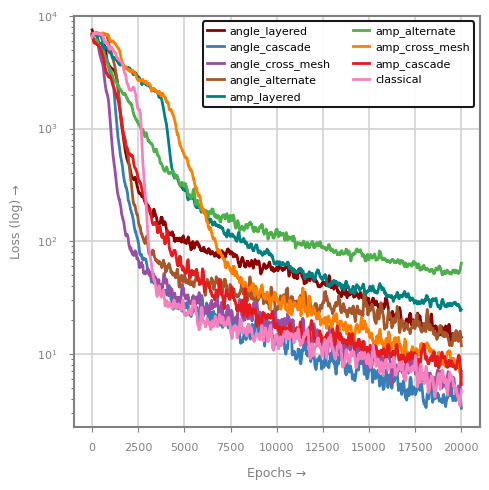
\includegraphics[width=0.4\columnwidth, trim={0cm 0cm 0cm 0cm}, clip]{figures/loss_history_helmholtz.png} 
    \caption{ Training loss history comparison for different models solving the Helmholtz equation. The plot shows convergence behaviour for angle-based, amplitude-based encodings for the circuits considered ( \textit{Cross-mesh}, \textit{Cascade}, \textit{Layered}, and \textit{Alternate}) and classical neural networks(Model-2) over 20,000 epochs.}
    \label{fig:loss_history_helmholtz}
\end{figure}

 
\begin{figure}[t]
    \centering
    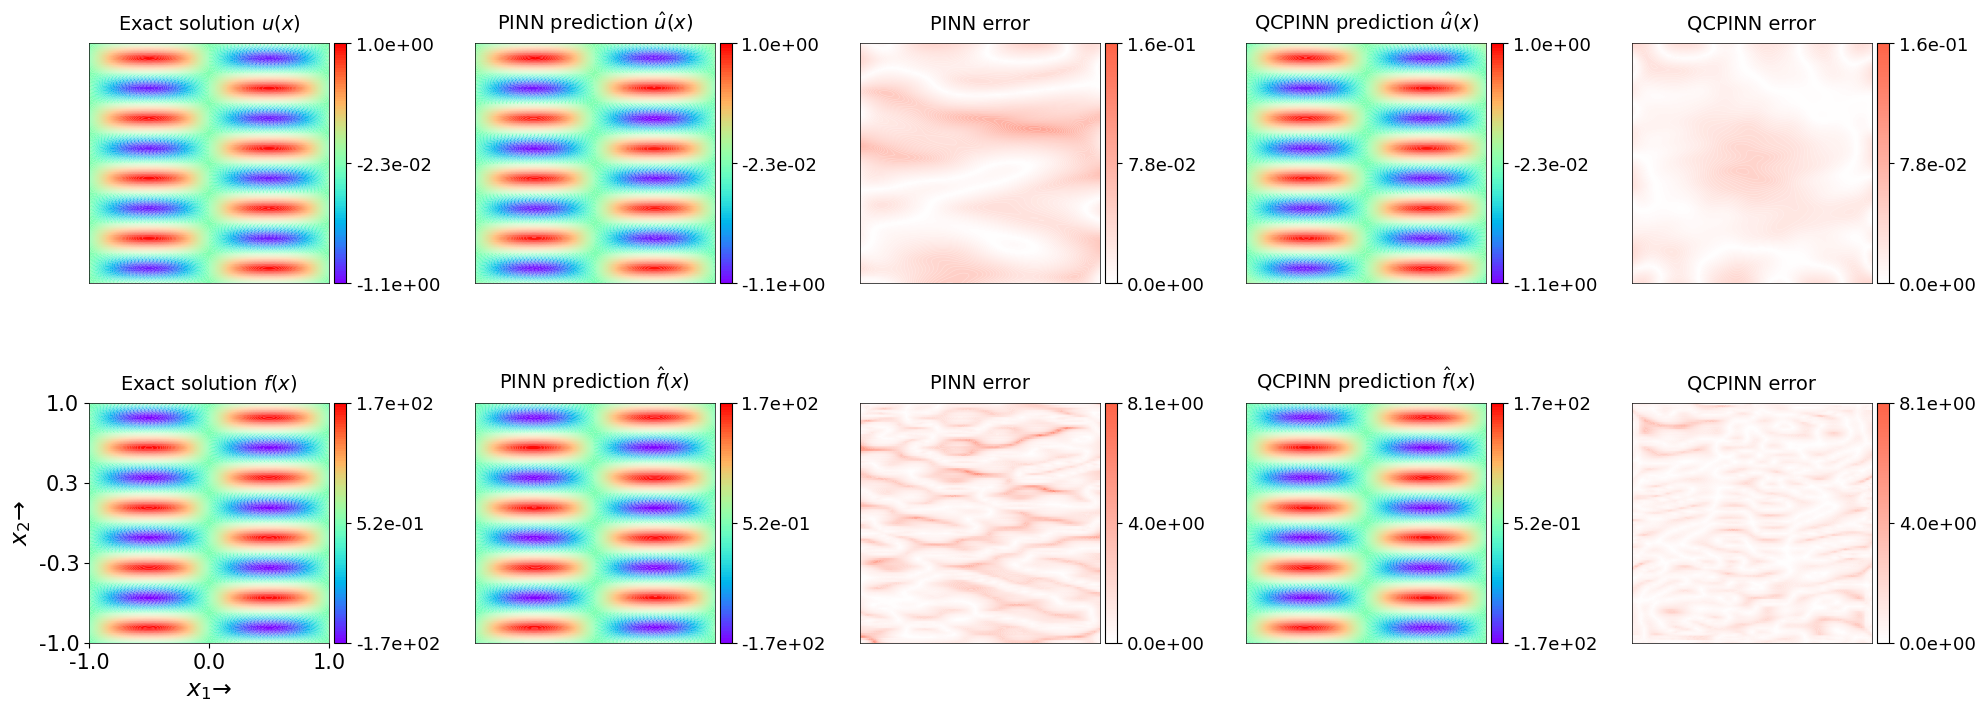
\includegraphics[width=0.85\columnwidth, trim={0.20cm 0.20cm 0.20cm 0.20cm}, clip]{figures/predition_helmholtz.png}     
    \caption{Comparison of the exact solution with classical neural network(Model-2) and angle-cascade QCPINN for the Helmholtz equation. In this figure, the first row is for the velocity field ($u$), and the second row is for the force field ($f$). 
    % Exact solution u(x), PINN prediction u(x), PINN error, QCPINN prediction u(x), QCPINN error 
    }
    \label{fig:helmholtz_prediction}
\end{figure}



\begin{table}[t]
\centering
\caption{Performance comparison of the hybrid QCPINN models for the Cavity problem (\ref{eq:Cavity}). The table presents the number of trainable parameters, relative $L_2$ error (\%), and final training loss.}
\label{tab:results_cavity}
\scriptsize
\begin{tabular}{@{}l
        c@{\hspace{8.0pt}}
        c@{\hspace{4.0pt}}@{\hspace{4.0pt}} |
        c@{\hspace{8.0pt}}
        c@{\hspace{8.0pt}}
        c@{\hspace{8.0pt}}
        c@{\hspace{8.0pt}}
        @{}}
        
\toprule
\multicolumn{3}{c|}{\textbf{Method}} &\textbf{\makecell{\# Trainable \\Parameters}} & \multicolumn{2}{l}\textbf{\makecell{Relative $L_2$\\ Error(\%)}} & \textbf{\makecell{Final Training\\  Loss}} \\
\midrule
  % \multirow{6}{*}{CV} & \multicolumn{2}{c|}{\multirow{2}{*}{Algorithm(\ref{alg:algorithm1})}} & \multirow{3}{*}{621} & u & $9.266e+01$  & \multirow{3}{*}{0.102} & \multirow{3}{*}{-}\\
  %                          &     &  & &   v &  $1.000e+02$ & &  \\
  %                          &     &  & &   p &  $9.273e+01$ & &  \\
  %       \cline{2- 7} \noalign{\vskip 1ex}
  %                          &      \multicolumn{2}{c|}{\multirow{3}{*}
  %                          {Algorithm(2)}} & \multirow{3}{*}{725} & u & $9.345e+01$  &  \multirow{3}{*}{0.341} &  \multirow{3}{*}{2600}\\
  %                          &     &  & &  v &  $9.979e+01$ & &  \\
  %                          &     &  & &  p &  $8.620e+01$ & &  \\
  %       \cline{1- 7} \noalign{\vskip 1ex}
          
                           \multirow{26}{*}{DV} &  \multirow{11}{*}{\makecell{Amplitude \\ Encoding}}    &   \multirow{3}{*}{\textit{Alternate}} & \multirow{3}{*}{933}  & u& $6.441e+01$ &  \multirow{3}{*}{0.127}\\
                           &     &  & &  v & $8.439e+01$ &   \\
                           &     &  & &  p & $6.102e+01$ &   \\
        \cline{3- 7} \noalign{\vskip 1ex}
                           &    &   \multirow{3}{*}{\textit{Cascade}} & \multirow{3}{*}{928}  & u& $6.670e+01$ &  \multirow{3}{*}{0.123}\\
                           &     &  & &  v &  $8.409e+01$ &  \\
                           &     &  & &  p &  $6.365e+01$ &  \\
        \cline{3- 7} \noalign{\vskip 1ex}
                           &  & \multirow{3}{*}{\textit{Cross-mesh}} & \multirow{3}{*}{988} & u& $7.073e+01$&  \multirow{3}{*}{0.109} \\
                           &     &  & &  v &  $4.893e+01$ & \\
                           &     &  & &  p &  $7.096e+01$ & \\
        \cline{3- 7} \noalign{\vskip 1ex}
                           && \multirow{3}{*}{\textit{Layered}} & \multirow{3}{*}{933} & u& $5.690e+01$&  \multirow{3}{*}{0.121} \\
                           &     &  & &  v &  $9.476e+01$ &  \\
                           &     &  & &  p &  $7.469e+01$ &  \\

        \cline{2- 7} \noalign{\vskip 1ex}

                           &  \multirow{11}{*}{\makecell{Angle \\ Encoding}}   &  \multirow{3}{*}{\textit{Alternate}} & \multirow{3}{*}{933}  & u& $4.041e+01$ &\multirow{3}{*}{0.109} \\
                           &     &  & &  v & $4.683e+01$ &    \\
                           &     &  & &  p & $4.746e+01$ &    \\
        \cline{3- 7} \noalign{\vskip 1ex}

                           &  & \multirow{3}{*}{\textit{Cascade}} & \multirow{3}{*}{928} & u & $ 2.745e+01$  &  \multirow{3}{*}{0.083} \\
                           &     &  & &  v &  $2.081e+01$ &   \\
                           &     &  & &  p &  $4.791e+01$ &  \\
        \cline{3- 7} \noalign{\vskip 1ex}
                             & \multirow{9}{*} & \multirow{3}{*}{\textit{Cross-mesh}} & \multirow{3}{*}{988} & u& $2.035e+01$ &  \multirow{3}{*}{ 0.084} \\ 
                           &     &  &  & v &  $2.071e+01$ &  \\
                           &     &  &  & p &  $4.011e+01$ &  \\
        \cline{3- 7} \noalign{\vskip 1ex}

                            & & \multirow{3}{*}{\textit{Layered}} & \multirow{3}{*}{933} & u& $4.572e+01  $ &  \multirow{3}{*}{0.129} \\ 
                           &     &  &  & v &  $6.628e+01$ & \\
                           &     &  &  & p &  $7.885e+01$ & \\

        \cline{1- 7} \noalign{\vskip 1ex}

                           \multirow{6}{*}{Classical}& \multicolumn{2}{c|}{\multirow{3}{*}{Model-1}}&\multirow{3}{*}{8003}  & u  & $2.103e+01 $& \multirow{3}{*}{0.087}  \\
                           &     &  & &  v &$3.027e+01 $& \\
                           &     &  & &  p &$ 2.317e+01 $& \\

        \cline{2- 7} \noalign{\vskip 1ex}

                           &\multicolumn{2}{c|}{\multirow{3}{*}{Model-2}}& \multirow{3}{*}{2903}  & u  & $3.830e+01$& \multirow{3}{*}{0.073}  \\
                           &     &  & &  v &$2.924e+01$& \\
                           &     &  & &  p &$4.106e+01$& \\
\bottomrule
\end{tabular}
\end{table}

\begin{figure}[t]
    \centering
    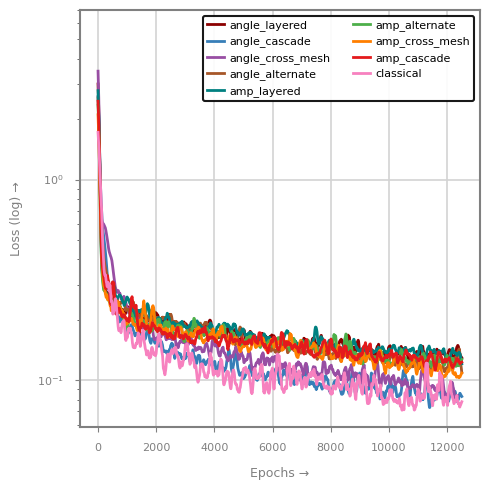
\includegraphics[width=0.4\columnwidth, trim={0cm 0cm 0cm 0cm}, clip]{figures/loss_history_cavity.png} 
    \caption{Training loss history comparison for different architectures solving the lid-driven cavity flow problem. The plot compares DV-based QCPINN with \textit{Cross-mesh}, \textit{Cascade}, \textit{Layered}, and \textit{Alternate} configurations for both amplitude and angle encodings, along with the Model-2 classical neural network results.}
    \label{fig:loss_history_cavity}
\end{figure}

\begin{figure}[t]
    \centering        
    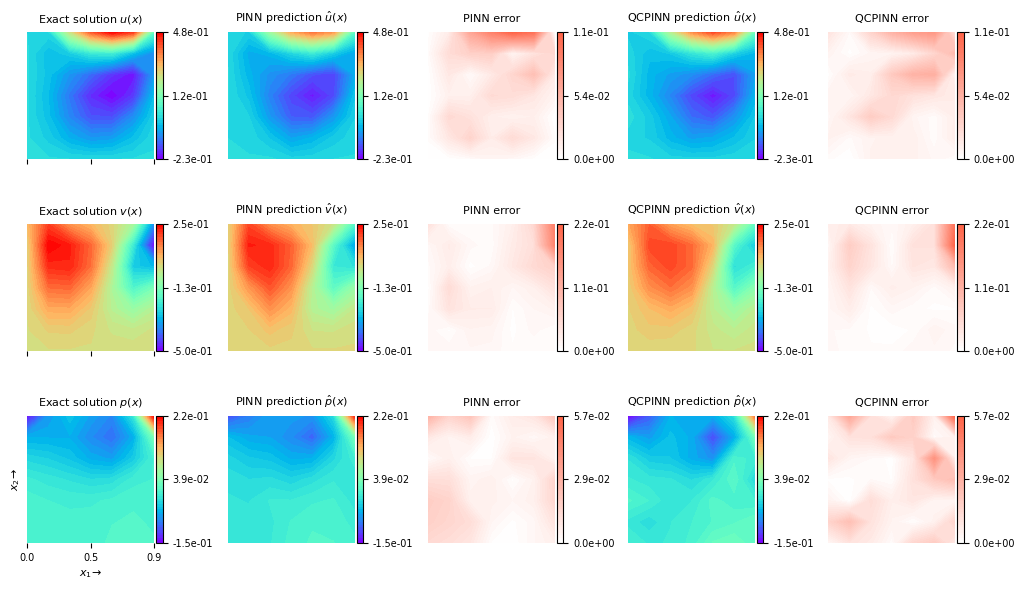
\includegraphics[width=0.85\columnwidth, trim={0cm 0.0cm 0cm 0.0cm}, clip]{figures/prediction_cavity.png} 
    \caption{  Cavity flow simulation results comparing exact solution with Model-2 classical and angle-cascade QCPINN predictions for velocity components (u, v) and pressure (p). The first row is exact solutions; the Second row is Model-1 classical neural network predictions; the Third row is an absolute error for classical predictions; the Fourth row is the angle-cascade QCPINN predictions; the Fifth row is an absolute error for angle-cascade QCPINN predictions.}
    \label{fig:cavity_prediction}
\end{figure}


\section{Results} \label{sec:results}

This section discusses the performance of the proposed CV-based and DV-based models and compares results with the classical models. For clarity in the following sections,  we refer to DV-based models using their encoding-architecture naming convention. For example, the term \textit{angle-cascade} QCPINN model specifically denotes a DV-based QCPINN model that employs the Cascade circuit with angle encoding.

The classical solver demonstrates stable training dynamics. As shown in Figures~\ref{fig:loss_history_helmholtz} and~\ref{fig:loss_history_cavity}, its training loss curves display smooth, monotonic convergence without significant oscillations. This stability stems from its well-understood optimization landscape and clear gradient flow path. The classical approach achieves competitive performance while maintaining consistent convergence across the Helmholtz and Cavity flow problems.
 
Experimental results show that CV quantum systems exhibit significant sensitivity to large values (see, for example, the residual loss of the Helmholtz equation in figure \ref{fig:cv_loss_plots}(a)), which can lead to numerical instability, loss of computational accuracy, and experimental challenges. 
%
The observed behaviour in figure \ref{fig:cv_loss_plots}, where the boundary condition (BC) loss decreases while the residual loss remains stagnant, can be attributed to the limitations of the CV quantum circuit in effectively approximating the solution function space. The small values required for stability in the squeezing, displacement, and Kerr parameters constrain the expressivity of the quantum layers, potentially limiting their ability to capture complex solution dynamics within the domain. As a result, the network prioritizes satisfying the boundary conditions, which are lower-dimensional constraints, while struggling to minimize the residual loss, which involves higher-order derivatives of the solution governed by the PDE. This suggests that alternative optimization strategies may be needed to improve overall convergence.
%
This heightened vulnerability to the complex optimization landscape was introduced by both Gaussian and non-Gaussian operations, as well as the PINN loss function. Consequently, CV models typically display slower training dynamics and necessitate careful parameter initialization to counteract gradient decay. 


While various normalization techniques were explored as potential solutions, they often led to information loss without significantly improving training stability. For instance, we initially implemented the Chebyshev feature mapping~\cite{oz2023efficient, kyriienko2021solving} to normalize the inputs, but this approach failed to yield meaningful improvements. Similarly, we experimented with random neural networks combined with Gaussian smoothing~\cite{dees2024unsupervised}, yet this method also proved ineffective. These challenges highlight the need for fundamentally different parameter optimization and stability control strategies tailored specifically to CV-based quantum systems.

The DV-based QCPINN models offer an intriguing middle ground. Although they lack the stability of the classical solver, they demonstrate significantly better training dynamics compared to CV approaches. The loss curves for various DV-based  QCPINN models in figure~(\ref{fig:loss_history_helmholtz}) and~(\ref{fig:loss_history_cavity}) reveal more controlled convergence patterns. While some oscillations are evident, they are considerably less severe than those in the CV-based QCPINN case. The different circuit architectures (\textit{Layered}, \textit{Alternate}, \textit{Cascade}, and \textit{Cross-mesh}) exhibit similar overall behaviour but vary in their convergence rates, indicating that the selection of quantum circuit architecture influences optimization stability while maintaining general training reliability. Moreover, amplitude encoding typically achieves faster initial convergence, though it tends to plateau at higher final loss values compared to angle encoding. This observation aligns with the findings of \cite{suzuki2020analysis}, which showed that amplitude encoding promotes rapid optimization by directly mapping data values to quantum states. Conversely, angle encoding can yield more stable long-term training performance. 


\subsection{Helmholtz Equation}
\label{subsec:results_helmholtz}

Table~(\ref{tab:results_helmholtz}) presents the performance of the DV-based QCPINN models we consider for solving the Helmholtz problem along with the classical models, evaluating them based on the number of trainable parameters, relative $L_2$ error, and final training loss. The results indicate that among these models, \textit{Cascade} consistently outperforms other quantum models, achieving the lowest final training loss (3.30 for angle encoding and 6.372 for amplitude encoding), along with low relative $L_2$ testing errors. This suggests that \textit{Cascade} provides better convergence for the Helmholtz problem. In contrast, the \textit{Layered} and \textit{Alternate} circuits show higher final training losses, especially for the \textit{Layered} model in amplitude encoding (39.44). The classical models achieve a final training loss of 4.77 ( Model-2), making it comparable to quantum models but with significantly higher parameter usage.

Figure~(\ref{fig:helmholtz_prediction}) compares solution fields for the Helmholtz equation, highlighting differences between the best classical results and angle-cascade QCPINN. The classical model captures the overall structure but introduces noticeable discrepancies, as the absolute error maps indicate, highlighting significant deviations near boundaries and regions of rapid variation. The angle-cascade QCPINN model's predictions closely align with the exact solutions while using fewer parameters than the classical approach. The corresponding error maps reveal a more uniform and lower magnitude error distribution, suggesting improved generalization and robustness of the QCPINN model.


\subsection{Time-dependent 2D id-driven Cavity Problem}

\label{subsec:results_cavity}

Table~(\ref{tab:results_cavity}) presents the performance of the proposed QCPINN methods for solving the Cavity problem. Among the DV-based QCPINN models, \textit{Cascade} achieves the 
best overall performance, with the lowest final training loss (0.083 for angle encoding and 0.123 for amplitude encoding), demonstrating its good convergence properties.  Angle-cross-mesh also performs well, achieving the lowest final training loss (0.084), highlighting its effectiveness in this setting. 
%
Despite having significantly more trainable parameters, the classical approach achieves a comparable final loss compared to these quantum models, indicating that quantum models can achieve similar accuracy with fewer parameters.

Figure~(\ref{fig:cavity_prediction}) compares the predictions of the lid-driven cavity flow with the exact solutions, the classical PINN network, and the angle-cascade QCPINN model. The visualization illustrates the three key flow variables: horizontal velocity (u), vertical velocity (v), and pressure (p) at a Reynolds number of Re = 100 ($\mu = 0.01$).
%
The first row displays the reference solution obtained through finite volume methods, capturing the characteristic features of the Cavity flow. The pressure field shows a gradient that drives the recirculating flow pattern, with significant pressure differences between the moving lid and the cavity corners.

The Model-1 classical PINN (second row) and the angle-cascade QCPINN (fourth row) effectively capture the main flow features, although with varying degrees of accuracy. The angle-cascade QCPINN model agrees with the exact solution in reproducing the complex structures of the velocity fields. This is especially clear when predicting the primary vortex's location and strength, where the quantum model preserves the correct asymmetric positioning characteristic of the cavity flow.

The absolute error distributions (third and fifth rows) reveal distinct patterns in both velocity components and pressure fields. Both models display higher errors near the moving lid (u=1) for the velocity components, where the flow experiences the most significant shear. The angle-cascade QCPINN model demonstrates improved prediction accuracy in the pressure field (p), especially in maintaining the correct gradient directions. Both models encounter challenges in pressure prediction near the corners where singular-like behavior occurs.

